%==============================================================================
%  FINAL PROJECT PAPER  (IEEE Conference format)
%  Category B: AI-agent code optimization on KernelBench
%  Main body + references <= 6 pages; Appendix (raw materials) excluded.
%  Compile with pdfLaTeX from the repository root (figures under report/figures/).
%==============================================================================
\documentclass[conference]{IEEEtran}
\IEEEoverridecommandlockouts

\usepackage{cite}
\usepackage{amsmath,amssymb,amsfonts}
\usepackage{algorithmic}
\usepackage{graphicx}
\usepackage{textcomp}
\usepackage{xcolor}
\usepackage{listings}
\usepackage{url}
\usepackage{booktabs}
\usepackage{microtype}          % protrusion + font expansion: much better justification
\usepackage[htt]{hyphenat}      % allow hyphenation inside \texttt{...} identifiers
\usepackage[hidelinks]{hyperref}

% --- page-budget check: records where the main body + references end, and
%     reminds you in the compile log if it exceeds the 6-page limit.
\newcommand{\mainbodyendpage}{?}
\AtEndDocument{%
  \typeout{====================================================}%
  \typeout{[PAGE BUDGET] Main body + references end on page \mainbodyendpage\space (limit: 6, Appendix excluded).}%
  \typeout{====================================================}%
}

% --- style for verbatim prompts / agent output in the Appendix
\lstset{
  basicstyle=\ttfamily\scriptsize,
  breaklines=true,
  frame=single,
  columns=fullflexible,
  showstringspaces=false,
  keepspaces=true,
  xleftmargin=0.5em
}

\begin{document}

\title{Correct First, Fast Second: What a Local 7B Code Model Can and Cannot Do\\
for GPU Kernel Optimization\\
{\footnotesize Final Project --- Parallel Programming, Spring 2026}}

\author{%
\IEEEauthorblockN{Eric Tsou}
\IEEEauthorblockA{B11902044 \\ Dept.\ of Computer Science and Information Engineering, National Taiwan University \\ tsouoeric@gmail.com}%
}

\maketitle

%------------------------------------------------------------------------------
\begin{abstract}
We study how much the \emph{interaction strategy} around a fixed, locally hosted
7B-parameter code model (Qwen2.5-Coder-7B-Instruct) affects its ability to replace
PyTorch operators with custom CUDA kernels. On 30 KernelBench tasks (levels 1--3,
first 10 each, evaluated on a V100), we compare four regimes of increasing
structure: zero-shot prompting, profiling-guided prompting, iterative refinement on
execution feedback, and a five-agent loop (analysis, retrieval, generation,
evaluation, feedback triage) built from the same model. Three findings stand out.
(1)~Correctness, not speed, is the binding constraint: even \emph{correct} generated
kernels average 0.97--0.99$\times$ the speed of eager PyTorch, because a 7B model
cannot out-write cuBLAS/cuDNN on dense GEMM and convolution; the only real wins are
fused memory-bound epilogues. (2)~The best strategy depends on difficulty:
profiling-guided prompting is strongest overall (43\% correct, 27\% faster than
baseline), but the agent loop is the \emph{only} method that solves any level-2
fusion problem (3/10 vs.\ 0/10 for all others). (3)~Na\"ive agentic scaffolding is
actively harmful---our first agent scored 3\% correct, \emph{below} zero-shot's
30\%---and the decisive repairs were matching the agent's ambition to the model's
competence and spending compute on best-of-$n$ sampling under a real execution
oracle (3\%$\to$33\% correct from $n{=}1$ to $n{=}8$), not on more reasoning steps.
\end{abstract}

\begin{IEEEkeywords}
GPU kernel optimization, large language models, CUDA, agentic systems, KernelBench, test-time compute
\end{IEEEkeywords}

\vspace{0.5em}
\noindent\fbox{\parbox{0.97\columnwidth}{\textbf{Project Category:}\quad
$\square$~\textbf{A} (Self-chosen topic)\qquad
$\boxtimes$~\textbf{B} (AI-agent code optimization)\\[2pt]
\footnotesize Tick exactly one. This tells reviewers which lens to apply.}}

%------------------------------------------------------------------------------
\section{Introduction}

Writing fast GPU kernels is expert work: a correct, performant CUDA kernel must
respect memory coalescing, shared-memory capacity, occupancy, and numerical
semantics simultaneously. Large language models (LLMs) promise to automate parts of
this work, and benchmarks such as KernelBench~\cite{kernelbench} formalize the task:
given a PyTorch reference module \texttt{Model}, produce a functionally identical
\texttt{ModelNew} that replaces operators with custom CUDA and runs faster.

Most published results on this task use frontier-scale proprietary models. This
paper asks a question closer to what a practitioner with fixed local hardware faces:
\emph{holding a single mid-size open-weight model constant, how much does the
prompting and agent scaffolding around it matter---and where exactly does it help or
hurt?} The model is the controlled variable; the four treatment conditions are
zero-shot prompting, profiling-guided prompting, iterative refinement, and a
multi-agent loop in which the \emph{same} model plays four roles (code analyzer,
retrieval researcher, kernel generator, feedback triager) around a real
compile-and-run evaluator.

Our contributions: (i)~a controlled $1{\times}4$ comparison on 30 KernelBench tasks
with compile / correctness / speedup metrics and a per-difficulty breakdown;
(ii)~evidence that no single strategy dominates---guided prompting wins overall and
on whole networks, while only the agent solves fused multi-operator problems;
(iii)~a root-cause analysis of \emph{why} the agent initially scored below
zero-shot, and a principled repair (competence-matched ambition plus best-of-$n$
sampling under an execution oracle) validated by a coherent component-ablation
study and a test-time-compute scaling curve; (iv)~an infrastructure lesson---LLM-generated
kernels can deadlock the GPU, so unattended evaluation requires hard
per-candidate timeouts.

%------------------------------------------------------------------------------
\section{Background and Related Work}

\textbf{Benchmark and dataset.} KernelBench~\cite{kernelbench} contains PyTorch
reference modules in difficulty levels: level~1 holds single operators (GEMM
variants, convolutions, elementwise ops), level~2 holds short \emph{fused} operator
sequences (e.g.\ \texttt{ConvTranspose2d}$\to$\allowbreak\texttt{BiasAdd}$\to$\allowbreak\texttt{Clamp}$\to$\allowbreak\texttt{Scale}), and
level~3 holds full architectures (MLPs, LeNet-5, AlexNet, \dots). Each task ships
\texttt{get\_inputs()} generators; a candidate passes if its outputs match the
reference within tolerance across randomized trials. We use the \textbf{first 10
problems of each of levels 1--3} (30 tasks): the subset keeps a full
$4$-method~$\times$~$8$-variant study tractable on shared GPUs ($\sim$350 model
runs with multi-trial timing) while still spanning three qualitatively different
difficulty regimes. The headline metric is \emph{fast\textsubscript{1}}: the
fraction of tasks both correct \emph{and} faster than eager PyTorch~\cite{kernelbench}.

\textbf{Baseline.} The performance baseline is eager PyTorch, whose
matmul/convolution dispatch to highly tuned cuBLAS/cuDNN kernels---a strong
baseline that, as we show, dominates what a 7B model can hand-write for
compute-bound operators.

\textbf{Model and agent tooling.} All generation uses
Qwen2.5-Coder-7B-Instruct~\cite{qwen25coder} served locally via HuggingFace
Transformers (fp16, multi-GPU workers; one GPU generates while a second evaluates).
No proprietary model or API is used anywhere. The agent framework is $\sim$1{,}500
lines of our own Python orchestrating the roles described in \S\ref{sec:method};
retrieval uses BM25 over a small curated corpus of CUDA optimization notes
(tiling, coalescing, epilogue fusion, \texttt{torch.utils.cpp\_extension} usage).

\textbf{Related work.} Our design draws on retrieval-augmented
generation~\cite{rag}, self-refinement from execution
feedback~\cite{selfrefine,selfdebug,reflexion}, and repeated sampling with a
verifier, whose effectiveness on code is well documented~\cite{alphacode,monkeys}.
Our results echo \cite{monkeys} in a harsher setting: with a weak generator and a
real compile-and-run verifier, sampling breadth beats reasoning depth.

%------------------------------------------------------------------------------
\section{Methodology}\label{sec:method}

All four methods share the same base task prompt (Appendix~A), model, decoding
budget (4096 new tokens), and evaluator; they differ only in the information and
control flow around generation.

\subsection{The four interaction regimes}

\textbf{Zero-shot.} The raw KernelBench prompt; greedy decoding; one attempt. This
is the capability floor.

\textbf{Guided.} We profile each \emph{reference} module with the PyTorch profiler
on the target GPU and inject its top operators by CUDA time into the prompt,
followed by a roofline-style rule we added after the pilot study (\S\ref{sec:fail}):
\emph{do not reimplement matmul/conv---cuBLAS/cuDNN already won; fuse the cheap
memory-bound epilogue instead}. One attempt, no loop.

\textbf{Iterative.} Up to three turns: generate, compile/check/time on the GPU,
feed a distilled error/timing report back, regenerate. The submitted kernel is the
best turn under a $(\textit{correct},\textit{compiled},\textit{speedup})$ ranking.

\textbf{Agentic.} A five-role loop, all roles played by the same model with
different system prompts (Appendix~B):
\begin{enumerate}
  \item \emph{Code Analyzer} -- names the operations, bottlenecks, and fusion
        opportunities; emits retrieval queries.
  \item \emph{RAG Researcher} -- retrieves from the documentation corpus and writes
        a cited optimization brief.
  \item \emph{Kernel Generator} -- writes \texttt{ModelNew}; samples $n$ candidates
        per turn (best-of-$n$).
  \item \emph{Evaluator} (non-LLM) -- compiles, checks correctness, times each
        candidate; keeps the best per turn.
  \item \emph{Feedback Analyzer} -- converts raw evaluator output into a diagnosis
        and a directive for the next turn.
\end{enumerate}
The loop runs up to three turns. Every component can be disabled independently,
which yields the ablation study in \S\ref{sec:ablation}.

\subsection{How we iterated on the agent}\label{sec:iterate}

Category~B asks how the agent was \emph{guided}; the honest answer is that our
first agent failed badly, and the iteration that fixed it is a result in itself
(full chronology in Appendix~D).

\textbf{Pilot (v1): 3\% correct, 33\% compile---below zero-shot.} The v1 generator
system prompt \emph{mandated} custom kernels (``replace PyTorch operators \dots
using \texttt{load\_inline} or Triton''), and the analyzer/researcher briefs
recommended tiling, shared memory, and warp reductions on every task. The 7B model
attempted ambitious hand-tiled CUDA it could not compile---e.g.\ calling
\texttt{load\_inline(sources=...)} (a keyword that does not exist) and mismatching
\texttt{PYBIND11\_MODULE} names, yielding \texttt{PyInit} import errors. The
feedback loop could not recover because each retry stayed in the same
over-ambitious mode; tellingly, a single-turn variant \emph{beat} the full loop.

\textbf{Repairs (v2).} Four changes, each motivated by an observed failure:
(1)~\emph{Competence-matched prompting}: every agent role is instructed to reach a
correct, compiling kernel first---reuse \texttt{torch} ops for the heavy compute,
fuse only the memory-bound epilogue---and to escalate to hand-written tiling only
once a correct baseline exists; the prompts also pin the exact
\texttt{load\_inline} signature the model kept hallucinating.
(2)~\emph{Best-of-$n$ sampling}: $n{=}4$ candidates per turn at temperature~0.7,
ranked by the real evaluator. (3)~\emph{Monotone turn selection}: the submitted
kernel is the best turn by $(\textit{correct},\textit{compiled},\textit{speedup})$,
so a later broken retry can never displace an earlier working kernel (this bug had
been silently degrading the iterative baseline too). (4)~\emph{Hard evaluation
timeouts}: each candidate is evaluated in a child process killed after 240\,s,
because generated kernels can deadlock the GPU---one such kernel stalled a
production run for 14 hours (\S\ref{sec:infra}).

%------------------------------------------------------------------------------
\section{Experimental Setup}

\textbf{Hardware/software.} Generation and evaluation run on nodes with 8$\times$
NVIDIA V100-SXM2-32GB (Volta, no fp32 tensor cores), CUDA 12.3, PyTorch 2.x, GCC
10. Workers pair GPUs: one serves the model, one evaluates kernels, so generation
never competes with timing.

\textbf{Measurement.} For each candidate: compile via
\texttt{torch.utils.cpp\_extension}; correctness over 5 trials with randomized
inputs (must match the reference within KernelBench's default tolerance); timing
via CUDA events over 10 trials after warm-up, in fp32. The speed baseline is the
eager-PyTorch reference time measured on the same GPU.

\textbf{Success criteria.} We report: \emph{compile rate}; \emph{correctness rate};
\emph{fast\textsubscript{1}} = correct \textbf{and} faster than eager PyTorch (the
success definition for this study); and \emph{geometric-mean speedup} over correct
samples. A task counts once per (method, task) cell; multi-turn/multi-sample
methods submit exactly one final kernel chosen by the evaluator, never by the LLM's
own judgment.

\textbf{Reproducibility.} One command reruns the full matrix
(\path{experiments/run_all_experiments.sh}); the report, tables, and figures
regenerate from raw eval JSON via a single script. Completed cells are skipped, so
the study is incrementally re-runnable.

%------------------------------------------------------------------------------
\section{Results}

\subsection{Headline comparison}

\begin{table}[t]
\caption{Four methods on 30 KernelBench tasks (levels 1--3). fast$_1$ = correct and
faster than eager PyTorch. Geo-mean speedup is over correct samples only.}
\label{tab:headline}
\centering
\begin{tabular}{lcccc}
\toprule
Method & Compile\% & Correct\% & fast$_1$\% & Geo-mean \\
\midrule
Zero-shot   & 70 & 30 & 13 & 0.98$\times$ \\
\textbf{Guided} & \textbf{77} & \textbf{43} & \textbf{27} & 0.99$\times$ \\
Iterative   & 67 & 30 & 10 & 0.98$\times$ \\
Agentic     & 73 & 30 & 10 & 0.97$\times$ \\
\bottomrule
\end{tabular}
\end{table}

Table~\ref{tab:headline}: profiling-guided prompting is the best single strategy,
lifting correctness 30\%$\to$43\% and \emph{doubling} fast$_1$ (13\%$\to$27\%) over
zero-shot at identical compute. Iterative refinement does not help this model:
blind ``retry with the error log'' rarely converts failures. The repaired agent
reaches parity in aggregate---but with a very different distribution of successes.

\subsection{Difficulty decides the winner}

\begin{table}[t]
\caption{Correct solutions out of 10, per difficulty level.}
\label{tab:levels}
\centering
\begin{tabular}{lccc}
\toprule
Method & L1 (single op) & L2 (fused seq.) & L3 (network) \\
\midrule
Zero-shot & 9 & 0 & 0 \\
Guided    & \textbf{10} & 0 & \textbf{3} \\
Iterative & 9 & 0 & 0 \\
Agentic   & 5 & \textbf{3} & 1 \\
\bottomrule
\end{tabular}
\end{table}

Table~\ref{tab:levels} is the central qualitative result. On L1, simpler is better
(zero-shot/guided: 9--10/10) and the agent's machinery \emph{hurts} (5/10): its
analyzer talks the model into unnecessary custom kernels where a one-line torch op
passes. On L2, the agent is the \textbf{only} method that scores at all (3/10 vs.\
0/10 everywhere else): explicit fusion analysis plus an execution-grounded loop is
exactly what multi-operator fusion rewards. On L3, guided profiling uniquely
succeeds (3/10) by pointing the model at the dominant layer. No method dominates
across difficulty.

\subsection{Component ablation and test-time compute}\label{sec:ablation}

\begin{table}[t]
\caption{Agentic component ablation. Every variant flips one component off against
the same best-of-4 backbone; $\Delta$ is correctness change vs.\ the full system.}
\label{tab:ablation}
\centering
\begin{tabular}{lcccc}
\toprule
Variant & Correct\% & Compile\% & fast$_1$\% & $\Delta$ \\
\midrule
\textbf{Agentic (full, $n{=}4$)} & 30 & 73 & 10 & --- \\
$-$ RAG researcher       & 20 & 77 & 7  & $-10$ \\
$-$ Code analyzer        & 20 & 63 & 10 & $-10$ \\
$-$ Feedback analyzer    & \textbf{37} & 73 & 10 & $\mathbf{+7}$ \\
$-$ Refinement loop      & 20 & 70 & 10 & $-10$ \\
$-$ Best-of-$n$ ($n{=}1$) & 3  & 23 & 0  & $\mathbf{-27}$ \\
\bottomrule
\end{tabular}
\end{table}

\begin{figure}[t]
  \centering
  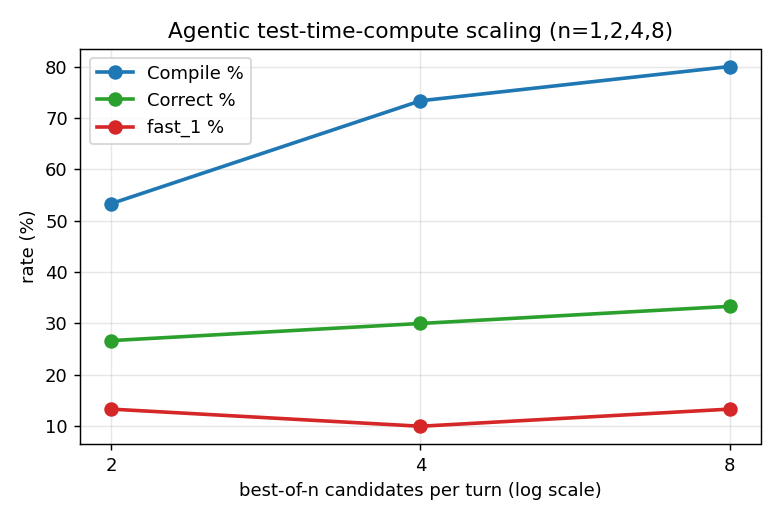
\includegraphics[width=\columnwidth]{report/figures/bestof_scaling.png}
  \caption{Test-time-compute scaling: full agent, varying only candidates per turn
  ($n\in\{1,2,4,8\}$; evaluator keeps the best). Correctness: 3/27/30/33\%;
  compile: 23/53/73/80\%. The first doubling is transformative; returns then
  diminish.}
  \label{fig:bestof}
\end{figure}

Table~\ref{tab:ablation} and Fig.~\ref{fig:bestof} decompose the agent.
\textbf{Best-of-$n$ is the load-bearing component by a wide margin}: removing it
collapses the system to 3\% correct / 23\% compile---\emph{worse than the
unrepaired pilot}. The analyzer, retrieval, and the loop each contribute
$\approx{+}10$pp, but only on top of the sampling backbone. The
\textbf{feedback analyzer is mildly harmful} ($+7$pp when removed): its rewritten
diagnoses sometimes over-specify the next attempt (e.g.\ directing the model to
keep refactoring an already-correct design, Appendix~C.3), whereas the raw compiler
error leaves the model freer to make the small fix. The scaling curve is steep then
saturating: $n{=}1{\to}2$ buys $+24$pp correctness, $n{=}4{\to}8$ only $+3$pp for
double the evaluation cost.

\subsection{Error taxonomy}

\begin{table}[t]
\caption{Failure category counts over 30 tasks (correct excluded; ``slow'' =
correct but not faster than baseline).}
\label{tab:taxonomy}
\centering
\begin{tabular}{lccccc}
\toprule
Method & compile & halluc.\ API & shape & wrong out & slow \\
\midrule
Zero-shot & 7 & 4 & 5 & 4 & 5 \\
Guided    & 5 & 6 & 3 & 3 & 5 \\
Iterative & 9 & 3 & 4 & 4 & 6 \\
Agentic   & 8 & 8 & \textbf{0} & 5 & 6 \\
\bottomrule
\end{tabular}
\end{table}

Table~\ref{tab:taxonomy}: the agent eliminates \emph{shape mismatch} entirely (its
analyzer's explicit shape/fusion reasoning works) but doubles \emph{hallucinated
API} (8 cases)---steered toward writing more custom code, the model more often
invents symbols, e.g.\ including the non-public header
\texttt{ATen/native/cudnn/utils.h} or calling \texttt{F.batch\_norm} from C++.
The residual bottleneck is API grounding, not planning.

%------------------------------------------------------------------------------
\section{Discussion and Analysis}\label{sec:fail}

\subsection{Root cause 1: the cuBLAS/cuDNN ceiling (why ``slow'' happens)}

Across \emph{all} methods, geometric-mean speedup of correct kernels is
0.97--0.99$\times$: correct kernels are on average slightly \emph{slower} than
eager PyTorch. This is structural, not incidental. The L1 GEMM tasks are large
($4096^2$ matrices), firmly compute-bound, and PyTorch dispatches them to cuBLAS
kernels with architecture-tuned tiling and double-buffering; a na\"ive
\texttt{load\_inline} kernel from a 7B model achieves a fraction of that
throughput, and even its ``correct'' attempts only tie by ultimately delegating to
\texttt{torch.matmul}. The genuine wins are exactly where theory predicts custom
code can win: \emph{memory-bound} epilogues and reductions. The agent's best
speedup (1.23$\times$) came on the skinny-$K$ GEMM
(\path{7_Matmul_with_small_K}), where cuBLAS is launch/utilization-bound;
guided's wins came from fusing bias/activation/clamp chains after convolutions,
cutting kernel launches and global-memory round-trips. Consequently the realistic
objective for a small model is \textbf{correct fused kernels at $\sim$1$\times$},
and methods separate on correctness, which is what our metrics show.

\subsection{Root cause 2: why every single-shot method scores 0/10 on level 2}

L2 tasks chain 3--5 operators. A passing \texttt{ModelNew} must either write one
fused kernel (hard: the pilot showed the model cannot reliably compile tiled
multi-op CUDA) or carefully replicate the reference semantics while fusing the easy
parts (subtle: e.g.\ \path{2_ConvTranspose2d_BiasAdd_...} applies a
\emph{learned} bias whose shape broadcasts differently than the conv's own bias).
Zero-shot/guided/iterative fail through one of two doors: ambitious fused CUDA that
does not compile, or torch-level rewrites that silently change semantics
(\emph{wrong output}, Table~\ref{tab:taxonomy}). The agent's analyzer names the
exact operator chain and its dataflow before generation, and the loop gets a second
chance after a semantic miss---together worth 3/10 where everything else gets 0.
Its own L2 successes are honest about the model's competence ceiling: the
representative solution (Appendix~C.1) keeps \texttt{ConvTranspose2d}/\allowbreak
\texttt{MaxPool} as torch ops and fuses \texttt{clamp+mean} into one pass---a
correct fusion at 1.01$\times$, not a heroic kernel.

\subsection{Root cause 3: why the pilot agent lost to zero-shot}

The v1 failure was not randomness; it was a \emph{systematic mismatch between the
scaffold's ambition and the model's competence}. The scaffold pushed every task
toward custom tiled CUDA; the model could not compile it; the loop reinforced
rather than repaired (each diagnosis suggested more optimization, not retreat); and
the selection logic could discard an earlier compiling kernel for a later broken
one. Each repair in \S\ref{sec:iterate} targets one of those mechanisms. The
ablation confirms the diagnosis quantitatively: with the sampling backbone removed
($n{=}1$), v2 falls right back to 3\%---i.e.\ the prompts alone do not fix a weak
generator; \emph{breadth under a real verifier} does. This is the paper's central
lesson for agent design: for small models on verifiable tasks, allocate compute to
candidates evaluated by an oracle before allocating it to reasoning about any
single candidate.

\subsection{Root cause 4: infrastructure---generated kernels can hang the GPU}
\label{sec:infra}

Two production runs stalled mid-study: a sampled kernel deadlocked at runtime
(an infinite loop in device code), and since KernelBench evaluates in-process and a
Python signal cannot interrupt a running CUDA kernel, one candidate wedged a worker
for 14 hours. We now evaluate every candidate in a child process with a hard 240\,s
wall-clock kill, scoring timeouts as failures. Anyone running LLM-generated GPU
code unattended needs this.

\subsection{Limitations}

30 tasks, one model, one seed: differences of 1--2 problems are within noise, so we
foreground large effects (3\%$\to$30\% repair; the 0-vs-3 L2 split; the
best-of-$n$ curve) over small gaps. Greedy decoding makes the three non-sampling
methods near-deterministic; sampling variance is characterized by the best-of-$n$
sweep itself. Results are fp32 on Volta---on GPUs with tensor cores the
library-dominance ceiling may shift. Findings about competence-matched scaffolding
are claimed for small models only.

%------------------------------------------------------------------------------
\section{Conclusion}

Holding a local 7B code model fixed, the interaction strategy around it changes
KernelBench outcomes as much as any prompt detail---but not monotonically with
sophistication. Profiling-guided prompting is the best overall (43\% correct, 27\%
faster-than-baseline); a multi-agent loop is uniquely able to solve fused level-2
problems but over-engineers trivial ones; and an unrepaired agent is worse than no
agent. The decisive design choices were matching ambition to competence and buying
correctness with best-of-$n$ sampling under a real execution oracle---test-time
compute, not deeper reasoning. Speed remains bounded by cuBLAS/cuDNN: the
deliverable a small model can realistically own is the correct fused
memory-bound kernel at parity, which is precisely where these methods differentiate.
Future work: difficulty-aware routing (guided for L1/L3, agentic for L2 would reach
53\% correct on this set), API-grounded decoding to attack the hallucination
bottleneck, and fine-tuning on the preference/reflection trajectories the agent
already logs.

%------------------------------------------------------------------------------
\begin{thebibliography}{00}
\bibitem{kernelbench} A.~Ouyang, S.~Guo, S.~Arora, A.~L.~Zhang, W.~Hu, C.~R\'e, and
A.~Mirhoseini, ``KernelBench: Can LLMs write efficient GPU kernels?,''
\emph{arXiv:2502.10517}, 2025.
\bibitem{qwen25coder} B.~Hui \emph{et al.}, ``Qwen2.5-Coder technical report,''
\emph{arXiv:2409.12186}, 2024.
\bibitem{rag} P.~Lewis \emph{et al.}, ``Retrieval-augmented generation for
knowledge-intensive NLP tasks,'' in \emph{NeurIPS}, 2020.
\bibitem{selfrefine} A.~Madaan \emph{et al.}, ``Self-Refine: Iterative refinement
with self-feedback,'' in \emph{NeurIPS}, 2023.
\bibitem{selfdebug} X.~Chen, M.~Lin, N.~Sch\"arli, and D.~Zhou, ``Teaching large
language models to self-debug,'' in \emph{ICLR}, 2024.
\bibitem{reflexion} N.~Shinn, F.~Cassano, E.~Berman, A.~Gopinath, K.~Narasimhan,
and S.~Yao, ``Reflexion: Language agents with verbal reinforcement learning,'' in
\emph{NeurIPS}, 2023.
\bibitem{alphacode} Y.~Li \emph{et al.}, ``Competition-level code generation with
AlphaCode,'' \emph{Science}, vol.~378, no.~6624, 2022.
\bibitem{monkeys} B.~Brown \emph{et al.}, ``Large language monkeys: Scaling
inference compute with repeated sampling,'' \emph{arXiv:2407.21787}, 2024.
\end{thebibliography}

% ---- end of main body + references. Everything below is the Appendix and is
%      NOT counted toward the 6-page limit. ----
\xdef\mainbodyendpage{\thepage}

%==============================================================================
%  APPENDIX -- REQUIRED RAW MATERIALS (Category B)
%  Verbatim input prompt, system prompts, representative agent output, and the
%  changes made to the agent. Complete artifacts (all 30 tasks x all methods:
%  prompts, generations, eval JSON, logs) are in the project repository under
%  experiments/runs/ and report/.
%==============================================================================
\appendices

\section{Input Prompt (verbatim)}

Base task prompt shared by all four methods, shown for level-1 problem~1
(\texttt{1\_Square\_matrix\_multiplication}); the architecture block changes per
task. Source: \texttt{data.json}.

\begin{lstlisting}
You write custom CUDA operators to replace the pytorch operators in the given architecture to get speedups.

You have complete freedom to choose the set of operators you want to replace. You may make the decision to replace some operators with custom CUDA operators and leave others unchanged. You may replace multiple operators with custom implementations, consider operator fusion opportunities (combining multiple operators into a single kernel, for example, combining matmul+relu), or algorithmic changes (such as online softmax). You are only limited by your imagination.

You are given the following architecture:

import torch
import torch.nn as nn

class Model(nn.Module):
    """
    Simple model that performs a single square matrix multiplication (C = A * B)
    """
    def __init__(self):
        super(Model, self).__init__()

    def forward(self, A: torch.Tensor, B: torch.Tensor) -> torch.Tensor:
        return torch.matmul(A, B)

N = 2048 * 2

def get_inputs():
    A = torch.rand(N, N)
    B = torch.rand(N, N)
    return [A, B]

def get_init_inputs():
    return []

Note: The kernels should be optimized for FP32 (32-bit floating point) precision.

Optimize the architecture named Model with custom CUDA operators! Name your optimized output architecture ModelNew. Output the new code in codeblocks. Please generate real code, NOT pseudocode, make sure the code compiles and is fully functional. Just output the new model code, no other text, and NO testing code!
\end{lstlisting}

\noindent The \emph{guided} method appends a profiling block before the final
instruction (excerpt; source: \texttt{guided/build\_prompt.py}):

\begin{lstlisting}
Here is GPU profiling information for the reference PyTorch implementation (measured on the target GPU):

Total CUDA time (reference forward): <X> ms
Top operators by CUDA time (self time when available):
  1. <op>: <t> ms
  ...

Use this profiling data to guide your optimization: focus on the highest-cost operators, consider kernel fusion where multiple hot ops appear in sequence, and target memory-bound vs compute-bound behavior implied by the dominant kernels.

Important: PyTorch already dispatches matmul/linear and convolution to highly tuned cuBLAS/cuDNN kernels -- a hand-written CUDA replacement for a plain GEMM or conv will almost always be SLOWER, not faster. Do not reimplement those from scratch. Instead, keep using the torch operator for the heavy compute and win by (1) fusing the cheap memory-bound epilogue around it (bias + activation + scale + clamp into one pass) and (2) replacing pure elementwise / reduction / normalization chains, where a custom kernel can actually cut memory traffic. Correctness first: only optimize an operator if you can keep the result numerically identical to the reference.
\end{lstlisting}

\section{System Prompts (verbatim, final v2)}

All four agent roles run on the same model. Source: \texttt{agentic/agents.py}.

\subsection{Code Analyzer}
\begin{lstlisting}
You are a senior GPU performance engineer. You analyse PyTorch reference modules and plan how to replace their operators with fast custom CUDA/HIP kernels. You are precise, concrete, and you never write the final kernel here.
\end{lstlisting}

\subsection{RAG Researcher}
\begin{lstlisting}
You are a research assistant for GPU kernel engineering. You are given retrieved documentation excerpts and must distil ONLY the techniques that are directly useful for the task. Ground every claim in the excerpts; never invent APIs. Cite the source tag (e.g. [memory_optimization.md#2]) after each point.
\end{lstlisting}

\subsection{Kernel Generator (the competence-matched v2 prompt)}
\begin{lstlisting}
You are an expert CUDA/HIP kernel engineer. Your FIRST priority is a ModelNew that compiles and matches the reference numerically; speed comes only after that. PyTorch already dispatches matmul/linear and convolution to highly tuned cuBLAS/cuDNN -- do NOT reimplement a plain GEMM or conv as a custom kernel, it will be slower. Keep the torch op for the heavy compute and add a custom kernel only where it clearly helps: fusing the memory-bound epilogue (bias/activation/scale/clamp) or replacing pure elementwise / reduction / normalization chains. When you do write a torch.utils.cpp_extension kernel, use load_inline(name=..., cpp_sources=..., cuda_sources=..., functions=[...]) -- note load_inline takes cpp_sources/cuda_sources, NOT a 'sources=' argument, and the pybind names in 'functions' must exactly match the C++ functions you define. Prefer one simple, correct fused kernel over several ambitious ones. You output ONLY a single ```python``` code block that defines class ModelNew(nn.Module) with the same interface as Model, plus get_inputs() and get_init_inputs(). No prose, no tests.
\end{lstlisting}

\noindent For comparison, the \textbf{v1 generator prompt} that produced the failed
pilot (3\% correct):
\begin{lstlisting}
You are an expert CUDA/HIP kernel engineer. You replace PyTorch operators with correct, high-performance custom kernels using torch.utils.cpp_extension (load_inline) or Triton. You output ONLY a single ```python``` code block that defines class ModelNew(nn.Module) with the same interface as Model, plus get_inputs() and get_init_inputs(). No prose, no tests.
\end{lstlisting}

\subsection{Feedback Analyzer}
\begin{lstlisting}
You are a debugging and performance triage expert for GPU kernels. Given an implementation and its evaluation result, you produce a crisp diagnosis and a concrete, prioritised fix list for the next attempt. You do NOT write the full kernel; you direct the fix.
\end{lstlisting}

\section{Representative Agent Output}

\subsection{A correct level-2 solution (the only method to solve any L2 task)}
Task \path{10_ConvTranspose2d_MaxPool_Hardtanh_Mean_Tanh}; final turn;
correct, 1.01$\times$. Note the competence-matched shape of the solution: torch ops
retained for conv/pool, \texttt{clamp+mean} fused into one pass.

\begin{lstlisting}
import torch
import torch.nn as nn
from torch.utils.cpp_extension import load_inline

class ModelNew(nn.Module):
    def __init__(self, in_channels, out_channels, kernel_size, stride, padding,
                 maxpool_kernel_size, maxpool_stride, hardtanh_min, hardtanh_max):
        super(ModelNew, self).__init__()
        self.conv_transpose = nn.ConvTranspose2d(in_channels, out_channels,
            kernel_size, stride=stride, padding=padding)
        self.maxpool = nn.MaxPool2d(kernel_size=maxpool_kernel_size,
            stride=maxpool_stride)
        self.hardtanh = nn.Hardtanh(min_val=hardtanh_min, max_val=hardtanh_max)

    def forward(self, x):
        x = self.conv_transpose(x)
        x = self.maxpool(x)
        x = self.fused_hardtanh_mean(x)
        x = torch.tanh(x)
        return x

    @staticmethod
    def fused_hardtanh_mean(x):
        return torch.mean(torch.clamp(x, min=-1, max=1), dim=(2, 3), keepdim=True)

def get_inputs():
    return [torch.rand(batch_size, in_channels, height, width)]

def get_init_inputs():
    return [in_channels, out_channels, kernel_size, stride, padding,
            maxpool_kernel_size, maxpool_stride, hardtanh_min, hardtanh_max]
\end{lstlisting}

\subsection{A representative failure (hallucinated API, $-$RAG variant)}
Compiler output excerpt; the model invented a private ATen header and called a
Python API from C++:

\begin{lstlisting}
fuse_relu_bn/cuda.cu:7:10: fatal error: ATen/native/cudnn/utils.h: No such file or directory
    7 | #include <ATen/native/cudnn/utils.h>

main.cpp:11:22: error: 'F' was not declared in this scope
   11 |  auto bn_output = F.batch_norm(x, weight, bias, running_mean, running_var, true, eps, 0.0);
main.cpp:19:56: error: 'fuse_relu_bn_cuda' was not declared in this scope
   19 | m.def("fuse_relu_bn_cuda", torch::wrap_pybind_function(fuse_relu_bn_cuda), ...);
\end{lstlisting}

\subsection{A Feedback Analyzer diagnosis (illustrating its failure mode)}
Produced after the already-correct turn~0 of the L2 task above; the directive
pushes further refactoring of a working design---the over-specification behavior
that makes removing this agent \emph{improve} correctness (Table~\ref{tab:ablation}):

\begin{lstlisting}
CATEGORY: performance
ROOT_CAUSE: The primary bottleneck identified is the `fused_hardtanh_mean` function, which involves both clamping and mean reduction operations. These operations are memory-bound and can benefit from being fused with subsequent operations to reduce the overall computational overhead.
DIRECTIVE: Refactor the ModelNew class to use the combined `fused_hardtanh_mean_tanh` function instead of the separate `fused_hardtanh_mean` function, and verify if the performance improves. Additionally, investigate any potential optimizations for the Convolution Transpose and Max Pooling operations.
\end{lstlisting}

\section{Changes Made to the Agent}

Chronological record of every modification, each motivated by an observed failure.
All code is in the project repository (\texttt{agentic/}, \texttt{experiments/}).

\textbf{C1. Generator/analyzer prompt inversion (``correct first'').}
v1 mandated custom \texttt{load\_inline}/Triton kernels for every task; v2
(Appendix~B.3) makes correctness the stated priority, forbids reimplementing plain
GEMM/conv, directs fusion to memory-bound epilogues, and pins the exact
\texttt{load\_inline} signature the model repeatedly hallucinated. The analyzer's
section instructions were rewritten the same way (flag matmul/conv as ``keep the
torch op''). \emph{Effect (with C2): 3\%$\to$30\% correct, 33\%$\to$73\% compile.}

\textbf{C2. Best-of-$n$ sampling under the execution oracle.}
The generator samples $n{=}4$ candidates per turn (temperature 0.7); the
\emph{evaluator}---not the LLM---ranks them by
$(\textit{correct},\textit{compiled},\textit{speedup})$ and keeps the best.
The ablation (Table~\ref{tab:ablation}) shows this is the single most important
component ($-27$pp when removed); the sweep (Fig.~\ref{fig:bestof}) maps
$n\in\{1,2,4,8\}$.

\textbf{C3. Monotone final-kernel selection.}
Previously the submitted kernel could be the \emph{last} generated turn even if an
earlier turn compiled and the last did not. Selection now maximizes
$(\textit{correct},\textit{compiled},\textit{speedup},\textit{turn})$ over all
turns, so refinement can never make the submission worse. (The same fix was applied
to the iterative baseline, for fairness.)

\textbf{C4. Hard per-candidate evaluation timeout.}
Each candidate is compiled/checked/timed in a child process killed after 240\,s
(\path{agentic/evaluator.py:evaluate_kernel_safe}). Motivation: a generated
kernel deadlocked the GPU and---because a Python signal cannot interrupt a running
CUDA kernel---wedged a worker for 14\,h. Timeouts are scored as ordinary failures.

\textbf{C5. Optional reference fallback (kept OFF for all reported numbers).}
A flag (\texttt{--fallback-to-reference}) can ship the unmodified reference
(\texttt{ModelNew = Model}) when no turn compiles---useful as a deployment floor,
but disabled throughout this study because a passthrough is trivially ``correct''
at 1$\times$ and would inflate benchmark correctness.

\textbf{C6. Coherent ablation infrastructure.}
All agentic variants share one best-of-4 backbone configuration
(\texttt{experiments/config.py}), so each ablation flips exactly one component;
the report generator renders the component table, the best-of-$n$ sweep, and the
scaling figure directly from raw evaluation JSON.

\end{document}
